% CVRB Research Paper – extended arXiv-ready version (≈3 pages)
% ---------------------------------------------------------------------------
\documentclass[11pt]{article}

% --- Packages --------------------------------------------------------------
\usepackage[margin=1in]{geometry}
\usepackage[T1]{fontenc}
\usepackage[utf8]{inputenc}
\usepackage{microtype}
\usepackage[hidelinks]{hyperref}
\usepackage{enumitem}
\usepackage{booktabs}
\usepackage{amsmath}
\usepackage{amsfonts}
\usepackage{amssymb}
\usepackage{graphicx}  % For \resizebox
\usepackage{float}    % For strict placement with [H]
\usepackage{placeins} % \FloatBarrier to keep tables in section
\usepackage{tikz}     % For programmatic diagrams
\usetikzlibrary{arrows.meta,positioning,calc}

% Compact lists
\setlist{nosep,leftmargin=*}

% Helper: shorten world names for wide table
\newcommand{\br}{\textsc{Binary-Ring90}}
\newcommand{\cw}{\textsc{Cipher}}
\newcommand{\cl}{\textsc{Chiral}}
\newcommand{\pf}{\textsc{Parity}}
\newcommand{\pfce}{\textsc{Prime}}
\newcommand{\fm}{\textsc{Fib}}
\newcommand{\ec}{\textsc{Elem}}
\newcommand{\cc}{\textsc{Chaos}}
\newcommand{\ms}{\textsc{Multi}}
\newcommand{\xorw}{\textsc{Xor}}
% Short names for additional worlds
\newcommand{\comets}{\textsc{Comets}}
\newcommand{\walkers}{\textsc{Walkers}}
\newcommand{\rten}{\textsc{Ring10}}
\newcommand{\dsra}{\textsc{DSRA}}
\newcommand{\mradix}{\textsc{MRadix}}
\newcommand{\nchains}{\textsc{NChains}}
\newcommand{\orbf}{\textsc{OrbForge}}
\newcommand{\pcoa}{\textsc{PCOA}}
\newcommand{\waver}{\textsc{WaveRing}}

% ---------------------------------------------------------------------------
\title{CVRB: A Code-Verified Reasoning Benchmark for\newline Self-Play World Generation}
\author{Yaron Lev \\ Independent Researcher \\ \texttt{yaron@pareto.sl}}
\date{}

\begin{document}
\maketitle

\begin{abstract}
Existing code\mbox{-}generation benchmarks such as \textbf{HumanEval} and \textbf{MBPP} probe short, self\mbox{-}contained functions whose correctness is checked by unit tests, so they rarely demand multi\mbox{-}step causal reasoning or long\mbox{-}horizon state tracking; they also rely on a fixed, human\mbox{-}curated task set that quickly saturates as models improve. \textbf{CVRB} moves beyond this limitation by letting LLMs \emph{themselves} create deterministic simulations (``worlds'') and corresponding questions, then independently regenerate the simulator via a second LLM to guarantee an unambiguous specification; this \emph{creator--validator duality} removes hidden test\mbox{-}case leakage. Because worlds are machine\mbox{-}generated and difficulty is tuned adaptively against a standing solver pool, the CVRB pipeline can be programmatically scaled as model capability increases - new, stronger models naturally produce harder tasks—while still yielding reproducible, code\mbox{-}verified scores.

\end{abstract}

% ---------------------------------------------------------------------------
\section{Introduction}
This paper introduces \textbf{CVRB~v0.1 (Pilot)}, a proof\mbox{-}of\mbox{-}concept release with ten validated worlds (50 questions) that demonstrates the feasibility of our fully automated pipeline. World creation, validation and solution checking are end\mbox{-}to\mbox{-}end executable; scores are obtained by running reference code, ensuring objectivity. On the pilot batch nine frontier models achieve $20$--$62\,\%$ accuracy, highlighting substantial headroom. Future releases will enlarge the benchmark automatically as both creators and solvers improve.


% ---------------------------------------------------------------------------


% ---------------------------------------------------------------------------
\section{Pipeline Overview}
The core CVRB engine is designed to run without human intervention via three isolated roles
implemented in Node.js (see \verb|server/src|):
\begin{description}
  \item[Creator] (\verb|create_worlds.js|) receives an LLM prompt (model,
        temperature, max length) and outputs \emph{(i)} a natural-language world
        description, \emph{(ii)} reference simulator code, and \emph{(iii)} JSON
        questions.
  \item[Validator] runs on a \emph{separate} LLM and receives only the natural-language description and JSON questions, never the Creator’s code. It regenerates the simulator from scratch, and only if the independent implementation matches bit-for-bit is the world stored in PostgreSQL with status \texttt{validated}. An exact match certifies that the specification is unambiguous to all readers.
  \item[Solver] (\verb|solve_world.js|) takes a world id, calls one or more
        LLMs in parallel and records the answer JSON alongside run-time
        metadata.  Scoring is deterministic: the server executes the Creator's
        reference code and compares outputs.
\end{description}


% Figures: Creator and Solver flows
\begin{figure}[H]
\centering
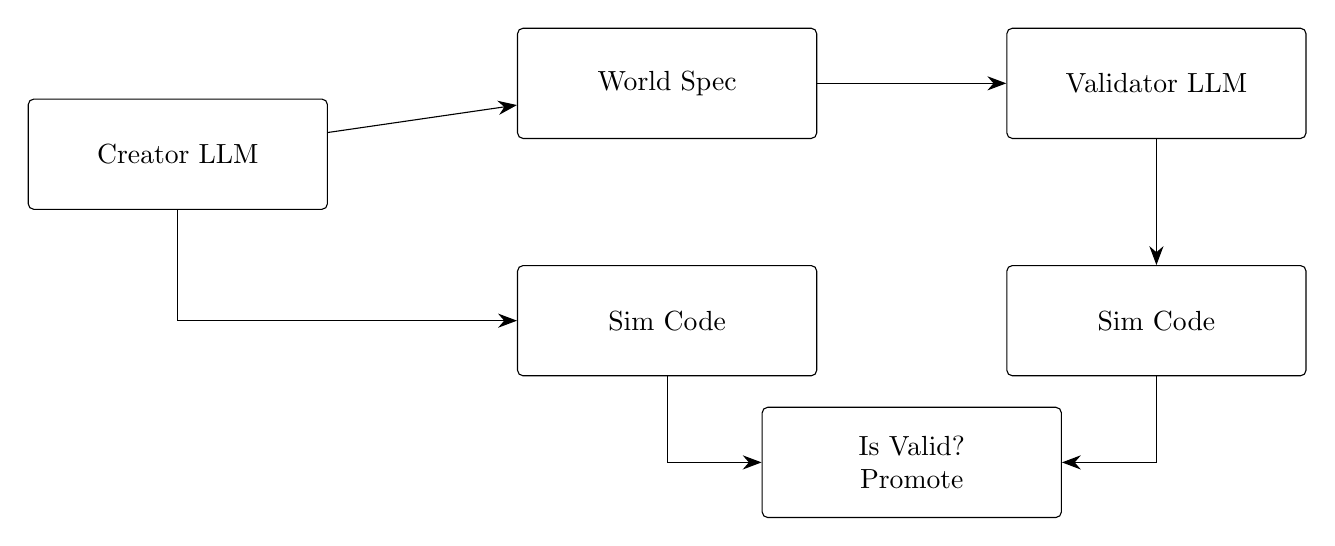
\begin{tikzpicture}[
  node distance=2.4cm,
  box/.style={draw, rounded corners=2pt, minimum width=3.8cm, minimum height=1.4cm, align=center},
  >={Stealth[length=2.4mm]}
]
  % Nodes
  \node[box] (creator) {Creator LLM};
  \node[box, right=of creator, yshift=0.9cm] (wspec) {World Spec};
  \node[box, below=1.6cm of wspec] (simA) {Sim Code};
  \node[box, right=of wspec] (validator) {Validator LLM};
  \node[box, below=1.6cm of validator] (simB) {Sim Code};
  \node[box] (promote) at ($ (simA)!0.5!(simB) + (0,-1.8) $) {Is Valid?\\Promote};

  % Flows
  \draw[->] (creator) -- (wspec);
  \draw[->] (creator) |- (simA);
  \draw[->] (wspec) -- (validator);
  \draw[->] (validator) -- (simB);
  \draw[->] (simA) |- (promote);
  \draw[->] (simB) |- (promote);
\end{tikzpicture}
\caption{Creator/Validator flow: the Creator produces a natural-language world specification and reference simulator code. A separate Validator LLM regenerates the simulator from the specification. If the two implementations match exactly, the world is accepted and promoted.}
\label{fig:creator-flow}
\end{figure}

\begin{figure}[H]
\centering
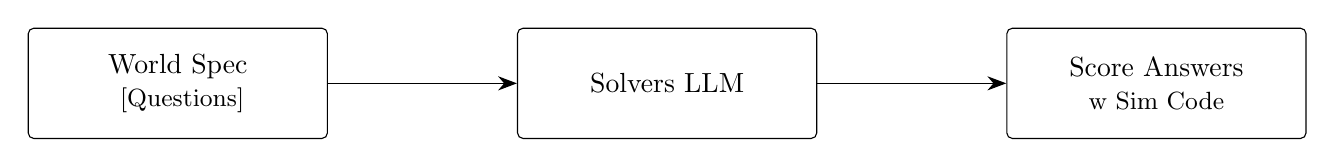
\begin{tikzpicture}[
  node distance=2.4cm,
  box/.style={draw, rounded corners=2pt, minimum width=3.8cm, minimum height=1.4cm, align=center},
  >={Stealth[length=2.4mm]}
]
  % Nodes
  \node[box] (spec) {World Spec\\\small{} [Questions]};
  \node[box, right=of spec] (solver) {Solvers LLM};
  \node[box, right=of solver] (score) {Score Answers\\\small{}w Sim Code};

  % Arrows
  \draw[->] (spec) -- (solver);
  \draw[->] (solver) -- (score);
\end{tikzpicture}
\caption{Solver flow: given a validated world specification and its question set, solvers produce answers that are scored deterministically by executing the reference simulator.}
\label{fig:solver-flow}
\end{figure}
\FloatBarrier

\paragraph{Selection pipeline.} For each Creator call, the scheduler generates \textbf{4--6 candidate worlds}. The Solver panel evaluates each candidate, we compute the \emph{quality score} (\S\ref{sec:quality}), and the system \emph{automatically} promotes the \textbf{top two per Creator} to the active benchmark set.

% ---------------------------------------------------------------------------
\section{Controlling Difficulty}
In v0.1, difficulty is set directly in the \textbf{Creator} prompt at question construction time. For each world the Creator must produce \textbf{five questions} that span a spectrum from very easy to very hard.

\paragraph{Prompt knobs.}
The prompt exposes concrete controls that shape difficulty:
\begin{itemize}
  \item \textbf{Brute-force steps:} approximate number of naive enumeration steps required if solved without insight.
  \item \textbf{Reasoning depth:} number of distinct logic jumps needed before a compact rule or shortcut is identified.
  \item \textbf{Simulation horizon:} number of forward simulation steps needed \emph{after} the logical rule is derived to reach the final answer.
\end{itemize}

The model is instructed that the \emph{very easy} question should be highly solvable by current solvers, while the \emph{hardest} should be effectively unsolvable for itself. Empirically this guidance produces a healthy spread of per-world difficulties, though a fuller analysis remains future work. 

% ---------------------------------------------------------------------------
\section{World Quality Score and Promotion}
\label{sec:quality}
CVRB now assigns each validated world a \emph{quality score} $q\in[0,1]$ computed directly from the distribution of solver accuracies:
\[
q = \frac{0.4\,\text{spread}+0.4\,\text{pair\_avg}+0.2\,\text{distinct}}{Q}.
\]
\begin{description}
  \item[spread] $=\max(\text{scores})-\min(\text{scores})$
  \item[pair\_avg] Mean absolute gap across every solver pair
  \item[distinct] Number of distinct score levels minus~1 (scores are given as %)
  \item[$Q$] The theoretical maximum (100 as percentages)
\end{description}
The weights \((0.4,0.4,0.2)\) were chosen heuristically to up-rank worlds that exhibit both a wide accuracy spread and multiple discrete score tiers across solvers.
This metric is a \emph{tunable pilot choice}: both the formula and the weights are exposed as configuration and may change in later versions as we gain empirical evidence about what best discriminates high-value worlds.
The implementation (\verb|server/src/CVRB/helpers/quality.js|) clamps the result to $[0,1]$ for numerical safety.

After scoring, the \textbf{promotion routine} (\verb|server/src/CVRB/helpers/world_promotion.js|) automatically promotes the \textbf{top two worlds per Creator} to benchmark set~1 in v0.1. The per-Creator budget and top-$K$ are configurable knobs intended for iteration.

% ---------------------------------------------------------------------------
\section{Benchmark Release v0.1: Dataset and Protocol}
The first public release ships \textbf{10 validated worlds}, each with exactly \textbf{5 questions} (50 in total). We asked \textbf{five reasoning--oriented LLMs} to act as Creators, two candidate worlds apiece. Only simulators that compiled and passed the Validator were kept. In preliminary pilots, general--purpose chat models produced fewer validated worlds, so for v0.1 we focused on reasoning--oriented models; this is a pragmatic pilot choice and will be revisited as we widen model coverage.

We included all major reasoning--oriented models in the Solver panel. In preliminary testing, general--purpose non--reasoning chat models achieved low but non--zero accuracy (e.g., GPT-4o around 15\% on v0.1); accordingly, the pilot analysis emphasizes reasoning--oriented models. A broader evaluation of non--reasoning models is left for future work. No additional filtering was applied to the reasoning--capable models.

The entire pipeline\,---Creator, Validator, solver evaluation, scoring and promotion---\,is orchestrated by a single scheduler script. Worlds that compile and pass validation are automatically scored (\S\ref{sec:quality}) and the promotion policy selects the public benchmark set with \emph{no human intervention}. All candidate worlds - accepted and rejected, remain in the GitHub repository and the public demo site for full transparency.

CVRB therefore functions as a \emph{relative leaderboard}: the active benchmark set evolves together with solver strength. Each snapshot (v0.1, v0.2\ldots) is frozen and archived to keep scores comparable within a version even as new worlds and creator models are added.

\paragraph{Security sandbox.} Every piece of LLM--generated JavaScript runs inside the \verb|node:vm| module with a 10~s wall--clock per question limit and no filesystem or network access, mitigating malicious payloads.
For complete mitigation, users can deploy the CVRB pipeline within a fully sandboxed environment.

% ---------------------------------------------------------------------------
\paragraph{Reproducibility.} The full backend\, front\-end and data artifacts are open\-sourced at \url{https://github.com/yaronl3v/CVRB}. During this pilot we queried all models via their default provider endpoints \emph{without} tuning temperature, top\-$k$ or other sampling knobs. No strict wall\-clock or token limits were imposed beyond the vendor defaults; if a model returned an error or no response at all the attempt was counted as a failure.

% ---------------------------------------------------------------------------
\section{Illustrative World: Fibonacci Modular Ring}
\label{sec:fib}
\textbf{Update rule.} A circular array of $N$ integers modulo a prime $P$. At every tick all cells update in parallel:
\[
  a'_i = (a_{i-1}+a_i) \bmod P ,
\]
with indices taken modulo $N$. The operation is linear over $\mathbb{Z}_P$ and therefore lends itself to matrix fast-doubling for $\mathcal{O}(N\log t)$ prediction.

\textbf{Edge cases.} $N{=}1$ reduces to $a'_0 = 2a_0 \bmod P$. For $P{=}2$ the rule becomes binary XOR. An all-zero ring remains zero; negative step counts are invalid.

\textbf{Worked example.} Initial state $[1,0,1,1]$, $P=5$, $t=3$ evolves as
\[
[1,0,1,1]\;\rightarrow\;[2,1,1,2]\;\rightarrow\;[4,3,2,3]\;\rightarrow\;[2,2,0,0],
\]
producing a final sum of~4.

% ---------------------------------------------------------------------------
\section{Experimental Results}
\label{sec:results}
\subsection{Aggregate accuracy}
\begin{table}[H]
\centering
\begin{tabular}{lcccc}
\toprule
Model & Correct & Accuracy & Beats Next & 95\,\% CI \\ \midrule
openai/o3                                 & 73 / 100 & 73\,\% & 98.4\,\% & $73\pm9$\,pp ($64$--$81$\,\%) \\
openai/o4-mini-high                       & 63 / 100 & 63\,\% & 79.4\,\% & $63\pm9$\,pp ($53$--$72$\,\%) \\
openai/gpt-5                              & 59 / 100 & 59\,\% & 79.1\,\% & $59\pm9$\,pp ($49$--$68$\,\%) \\
google/gemini-2.5-pro                     & 55 / 100 & 55\,\% & 96.5\,\% & $55\pm10$\,pp ($45$--$64$\,\%) \\
anthropic/claude-sonnet-4                 & 46 / 100 & 46\,\% & 65.6\,\% & $46\pm10$\,pp ($37$--$56$\,\%) \\
deepseek/deepseek-r1-0528                 & 44 / 100 & 44\,\% & 84.5\,\% & $44\pm10$\,pp ($35$--$54$\,\%) \\
qwen/qwen3-235b-a22b-thinking-2507        & 39 / 100 & 39\,\% & 94.2\,\% & $39\pm9$\,pp ($30$--$49$\,\%) \\
anthropic/claude-opus-4                   & 15 / 50  & 30\,\% & 81.8\,\% & $30\pm12$\,pp ($19$--$44$\,\%) \\
x-ai/grok-4                               & 25 / 100 & 25\,\% & 59.2\,\% & $25\pm8$\,pp ($18$--$34$\,\%) \\
google/gemini-2.5-flash                   & 24 / 100 & 24\,\% & 95.9\,\% & $24\pm8$\,pp ($17$--$33$\,\%) \\
openai/gpt-4o                             & 17 / 100 & 17\,\% & -- & $17\pm7$\,pp ($11$--$26$\,\%) \\
\bottomrule
\end{tabular}
\caption{Overall solver accuracy on the current benchmark; 95\,\% CIs shown. Sample sizes differ by model.}
\end{table}
\FloatBarrier

\subsection{Per-world breakdown}
\begin{table}[H]
\centering
\resizebox{\textwidth}{!}{%
\begin{tabular}{lcccccccccc}
\toprule
Model & \br & \cw & \cl & \pf & \pfce & \fm & \ec & \cc & \ms & \xorw \\ \midrule
o3                       & 80 & 40 & 60 & 100 & 40 & 60 & 60 & 60 & 80 & 40 \\
o4-mini-high             & 100 & 20 & 40 & 80 & 40 & 40 & 60 & 40 & 80 & 20 \\
gemini-2.5-pro           & 40 & 20 & 0 & 60 & 20 & 20 & 60 & 20 & 80 & 60 \\
deepseek-r1-0528         & 20 & 0 & 20 & 60 & 0 & 0 & 80 & 20 & 80 & 60 \\
claude-opus-4            & 60 & 0 & 0 & 20 & 0 & 20 & 60 & 40 & 80 & 20 \\
claude-sonnet-4          & 40 & 0 & 0 & 20 & 0 & 0 & 80 & 60 & 60 & 40 \\
grok-4                   & 60 & 0 & 0 & 20 & 0 & 20 & 80 & 40 & 40 & 20 \\
qwen3-235b-a22b-thinking-2507 & 20 & 0 & 0 & 80 & 0 & 0 & 60 & 40 & 40 & 20 \\
gemini-2.5-flash         & 40 & 0 & 0 & 20 & 0 & 0 & 60 & 40 & 40 & 0 \\
\bottomrule
\end{tabular}}\caption{Accuracy (\%) per model per world. Columns use abbreviated world names.}
\end{table}

% Additional per-world breakdown for new worlds
\begin{table}[H]
\centering
\resizebox{\textwidth}{!}{%
\begin{tabular}{lccccccccc}
\toprule
Model & \comets & \walkers & \rten & \dsra & \mradix & \nchains & \orbf & \pcoa & \waver \\ \midrule
o3                                          & 40 & 80 & 80 & 80 & 80 & 80 & 80 & 80 & 80 \\
o4-mini-high                                & 80 & 0  & 100 & 100 & 100 & 100 & 80 & 40 & 80 \\
gpt-5                                       & 80 & 20 & 40 & 40 & 100 & 100 & 80 & 60 & 80 \\
gemini-2.5-pro                              & 80 & 40 & 80 & 80 & 100 & 100 & 80 & 40 & 60 \\
claude-sonnet-4                             & 60 & 20 & 40 & 60 & 100 & 100 & 80 & 60 & 40 \\
deepseek-r1-0528                            & 60 & 0  & 0  & 60 & 100 & 40 & 100 & 40 & 80 \\
qwen3-235b-a22b-thinking-2507               & 60 & 0  & 20 & 60 & 100 & 80 & 80 & 20 & 60 \\
grok-4                                      & 80 & 0  & 20 & 0  & 0  & 60 & 20 & 40 & 0  \\
gemini-2.5-flash                            & 40 & 0  & 20 & 0  & 40 & 40 & 60 & 20 & 40 \\
gpt-4o                                      & 20 & 20 & 0  & 20 & 0  & 20 & 20 & 20 & 40 \\
\bottomrule
\end{tabular}}
\caption{Per-model accuracy (\%) on additional worlds. Columns use abbreviated world names.}
\end{table}

% ---------------------------------------------------------------------------
\section{Related Work}
Prior self-play benchmarks such as \emph{Sol-Ver}~\cite{sol-ver} and \emph{Self-Questioning LMs}~\cite{sqlm} generate tasks and check answers via unit tests or majority vote, but lack independent re-implementation. \emph{Code-as-Task}~\cite{code-as-task} focuses on tool use, and the \emph{Code World Models Benchmark}~\cite{cwmb} ships fixed environments. CVRB uniquely combines (i) model-generated deterministic simulations and (ii) dual independent implementations for consistency.

% ---------------------------------------------------------------------------
\section{Current Limitations}
\label{sec:limitations}
\begin{itemize}
  \item \textbf{Prompt-driven difficulty.} Difficulty is set entirely by prompt specifications; a more robust and automated solution is desirable.
  \item \textbf{World uniqueness.} The current version does not yet filter near-duplicate simulators; a semantic de-duplication pass is planned for the next release.
  \item \textbf{Theme breadth.} All existing worlds follow a ``deterministic step $+$ exploitable shortcut'' pattern (see the Creator prompt in \verb|world-creation.txt|). Future versions will introduce additional themes such as graph traversal, probabilistic processes and resource optimisation to widen the reasoning spectrum.
\end{itemize}

% ---------------------------------------------------------------------------
\section{Future Work}
\label{sec:future}
\begin{itemize}
  \item \textbf{Adaptive difficulty control.} The orchestrator can be extended to monitor solver accuracies and automatically adjust the Creator’s complexity levers (entity count, rule branching, time horizon) to target a balanced spread.
  \item \textbf{Template-driven diversity.} Richer \emph{world prompt templates} will encourage qualitatively different physics, objectives and edge cases, expanding the benchmark far beyond the ten v0.1 pilot worlds.
  \item \textbf{Uniqueness and coverage analysis.} We plan to cluster simulator kernels into semantic categories (e.g., cellular automata, graph processes, arithmetic puzzles) and enforce de-duplication within each bucket, ensuring the benchmark measures breadth rather than proficiency on near-duplicates.
\end{itemize}

\bibliographystyle{unsrt}
\bibliography{refs}

% ---------------------------------------------------------------------------
\section{Conclusion}
CVRB (\url{https://CVRB.dev}) offers an evergreen, code-verified benchmark for
algorithmic reasoning.  All source code is Apache-licensed on GitHub
(\url{https://github.com/yaronl3v/CVRB}).  We invite the community to contribute
solver agents, creator prompts, and new analysis tools.

\end{document}
